\documentclass[border=3pt,tikz]{standalone}
% Shared look for every TikZ figure in these notes.
% Included by each standalone figure file; also keeps the figures consistent
% with the colours used in the PDF and on the website.

\usepackage{tikz}
\usepackage{pgfplots}
\pgfplotsset{compat=1.18}
\usetikzlibrary{arrows.meta, decorations.markings, decorations.pathmorphing,
                patterns, calc, positioning}
\usepackage{amsmath}

% Series colours are the three validated categorical slots also used by the
% interactive widgets, so a path drawn in the printed notes and the same path on
% the website are the same colour. They clear the colour-vision-deficiency and
% contrast checks as a set; every path is direct-labelled as well, so colour is
% never the only thing carrying identity.
\definecolor{duPurple}{HTML}{68246D}
\definecolor{duBlue}{HTML}{2A78D6}
\definecolor{duRed}{HTML}{EB6834}
\definecolor{duGreen}{HTML}{1BAF7A}
\definecolor{duGrey}{HTML}{4D4D4D}

\tikzset{
  % heavier default lines and arrow tips, so diagrams stay clear when zoomed
  every picture/.append style = {line width=0.7pt, >={Stealth[length=3mm]}},
  axisline/.style   = {-{Stealth[length=3.4mm]}, line width=1.0pt, black},
  path1/.style      = {duBlue,   line width=1.6pt},
  path2/.style      = {duRed,    line width=1.6pt},
  path3/.style      = {duGreen,  line width=1.6pt},
  statedot/.style   = {circle, fill=black, inner sep=1.8pt},
  arrowhead/.style  = {decoration={markings,
                        mark=at position #1 with {\arrow{Stealth[length=3.4mm]}}},
                       postaction={decorate}},
  lbl/.style        = {font=\normalsize},
  slbl/.style       = {font=\small, duGrey},
  workfill/.style   = {duPurple, opacity=0.16},
}

% larger labels in plots as well
\pgfplotsset{every axis/.append style={label style={font=\normalsize}, tick label style={font=\small}, line width=0.9pt}}

% Textbook flow-work figure (868 x 308 px) with the board sketch on top:
% inlet  - the imaginary piston (green) pushes the fluid element (red) into the
%          control volume, to where the dotted element is;
% exit   - the fluid in the control volume (dotted) pushes the element (red)
%          out, and it in turn pushes the fluid ahead of it (blue piston).
\begin{document}
\begin{tikzpicture}[
    elem/.style={draw=duRed, line width=1.3pt, fill=duRed, fill opacity=0.35},
    ghost/.style={draw=duBlue, line width=1.1pt, densely dotted},
    rod/.style={line width=1.6pt, line cap=round}]
  \node[anchor=north west, inner sep=0] (img) at (0,0)
    {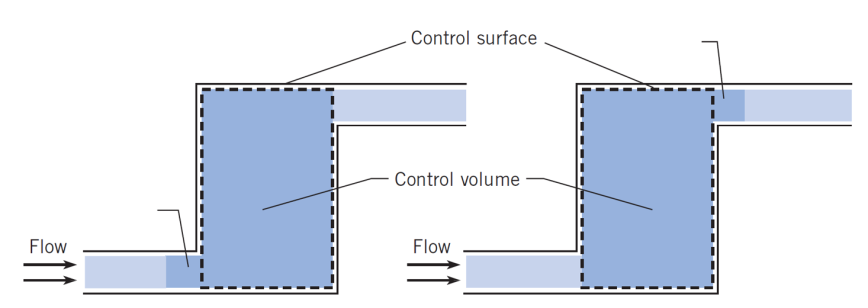
\includegraphics[width=11.7cm]{../img/ch4-flow-work-clean.png}};
  \begin{scope}[shift={(img.north west)}, x=11.7cm/868, y=-11.7cm/868]
    % ---- inlet
    \draw[elem] (167,258) rectangle (197,285);
    \draw[ghost] (205,258) rectangle (235,285);
    \fill[duGreen, draw=duGreen!70!black, line width=0.6pt] (152,258) rectangle (162,285);
    \draw[rod, duGreen] (152,271.5) -- (92,271.5);
    \node[duGreen!70!black, align=center, font=\small] (ip) at (78,178)
      {imaginary\\piston};
    \draw[-{Stealth[length=2.2mm]}, duGreen!70!black, line width=0.9pt]
      (ip.south) ++(12,0) .. controls (95,230) and (125,235) .. (150,255);
    % ---- exit
    \draw[ghost] (683,91) rectangle (709,119);
    \draw[elem] (719,91) rectangle (745,119);
    \fill[duBlue, draw=duBlue!70!black, line width=0.6pt] (750,91) rectangle (760,119);
    \draw[rod, duBlue] (760,105) -- (835,105);
  \end{scope}
\end{tikzpicture}
\end{document}
